% !TEX root = deplump.tex
\section{Experiments}
\label{sec:experiments}

The empirical performance of Deplump was evaluated using the most recent Wikipedia content dump as a test corpus.  

The mean number of recursions per byte incorporated into the model with a depth of 16 is 8.7326 (based on a 100K subsample of 100M byte sequence) and with a depth of 1024 the mean number of recursions is 9.0612.

\begin{figure*}[t] 
	\begin{center}
		\scalebox{1}{\includegraphics{figs/varying_depths.pdf}} % [clip=true, viewport= 1in 1in 9in 9in]
		\caption{Performance averaged over 10 random sections  100Mb sections of the corpus for varying fixed depths and number of allowable nodes ($L$) }
		\label{fig:varying_depths}
	\end{center} 
\end{figure*} 

\begin{figure*}[t] 
	\begin{center}
		\scalebox{.6}{\includegraphics{figs/varying_max_customers.pdf}} % [clip=true, viewport= 1in 1in 9in 9in]
		\caption{Performance for varying max allowable customers $k$.}
		\label{fig: varying_max_customers}
	\end{center} 
\end{figure*} 

\begin{figure*}[t] 
	\begin{center}
		\scalebox{.6}{\includegraphics{figs/varying_stream_length.pdf}} % [clip=true, viewport= 1in 1in 9in 9in]
		\caption{Performance for varying stream lengths and number of allowable nodes ($L$).}
		\label{fig:varying_stream_length}
	\end{center} 
\end{figure*} 

\begin{figure*}[t] 
	\begin{center}
		\scalebox{.45}{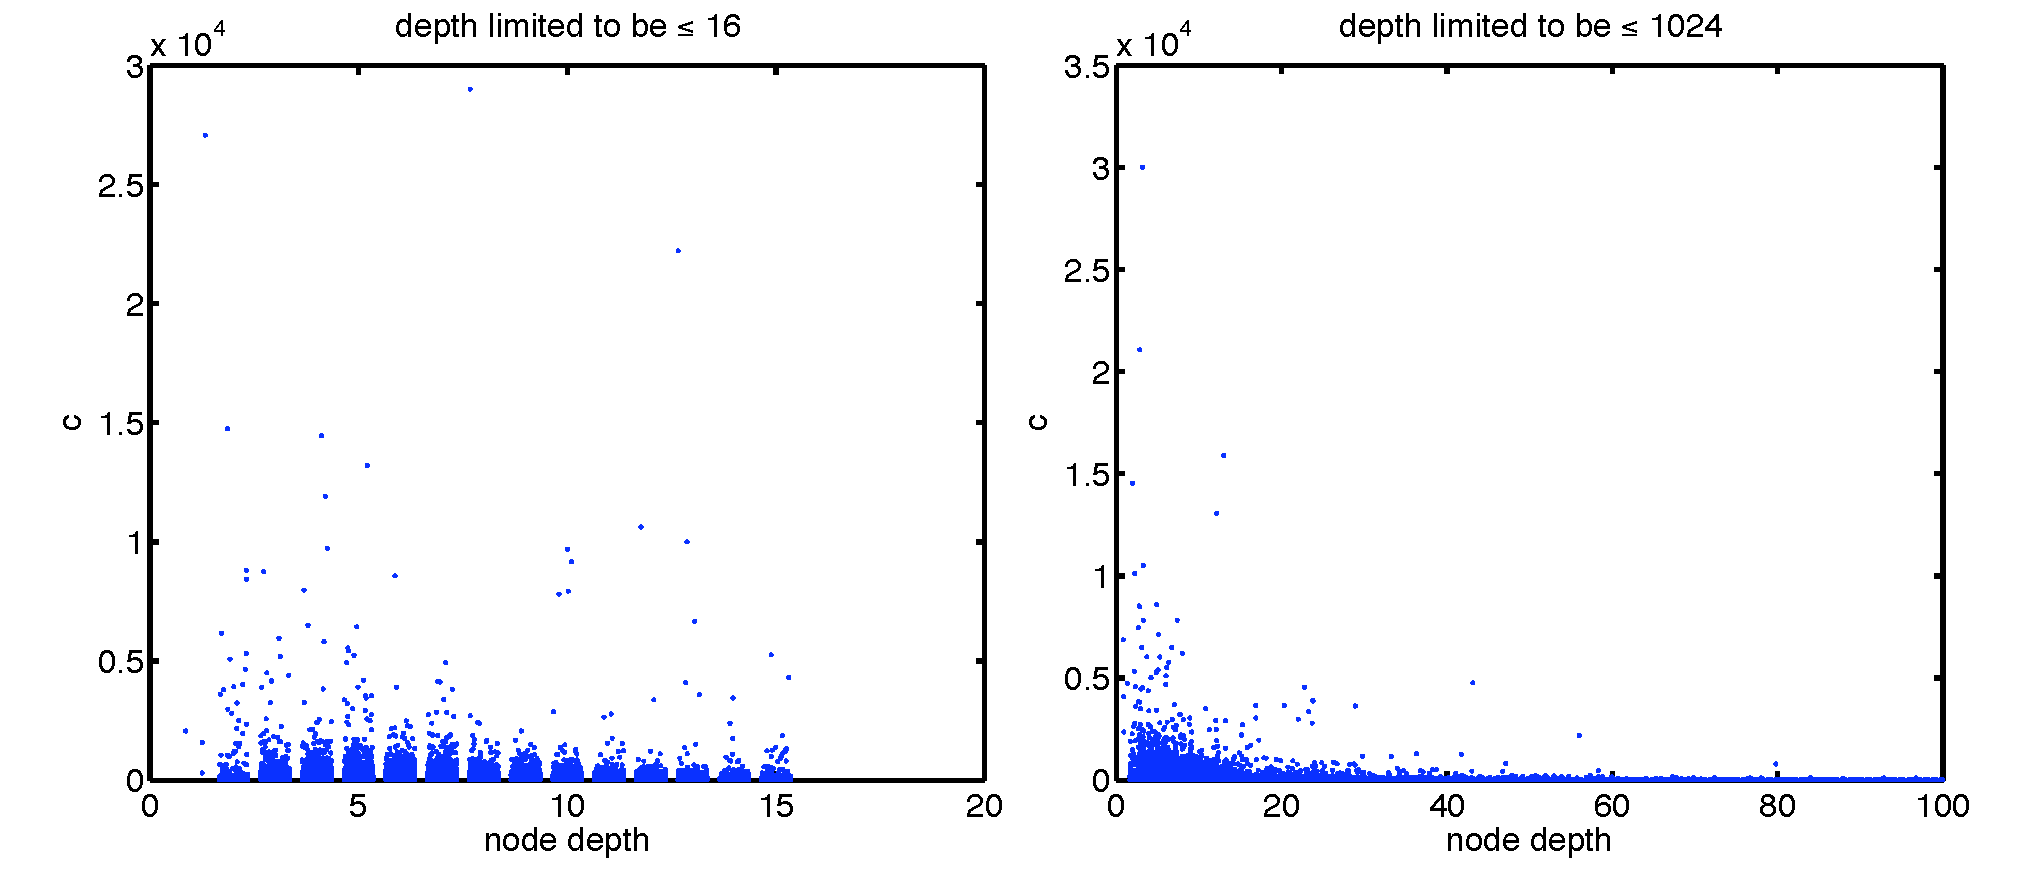
\includegraphics{figs/restaurant_plots.pdf}} % [clip=true, viewport= 1in 1in 9in 9in]
		\caption{Scatter plots to explore the relationship between the depth of a node and the total count}
		\label{fig:restaurant_plots}
	\end{center} 
\end{figure*} 
